% =====================================================================
%  Safe market probing with active power for sequential topology
%  discrimination in LV distribution grids
%  Method and formulas (paper-style draft v3), 2026-11-19
%  Source of truth for text and case data: ../MANUSCRIPT.md
%  The derivation outline (Sec. II, with the table that traces every
%  term of the final subproblem) and the proofs (Appendix) exist only
%  in this file.
%  Compile with pdfLaTeX (e.g. on Overleaf). No external .bib needed.
% =====================================================================
\documentclass[journal,onecolumn,11pt]{IEEEtran}

\usepackage{amsmath,amssymb}
\usepackage{bm}
\usepackage{booktabs}
\usepackage{array}
\usepackage{algorithm}
\usepackage{algpseudocode}
\usepackage{url}
\usepackage{tikz}
\usetikzlibrary{positioning,arrows.meta}
\usepackage[hidelinks]{hyperref}

\newtheorem{lemma}{Lemma}
\newtheorem{proposition}{Proposition}
\newtheorem{remark}{Remark}

\DeclareMathOperator{\vect}{vec}
\DeclareMathOperator{\diag}{diag}
\newcommand{\E}{\mathbb{E}}
\newcommand{\R}{\mathbb{R}}
\newcommand{\tp}{^{\top}}
\newcommand{\Nrm}{\mathcal{N}}
\newcommand{\dev}{\mathrm{dev}}

\begin{document}

\title{Safe Market Probing with Active Power for Sequential\\ Topology Discrimination in Low-Voltage Distribution Grids}
\author{Draft v3 of 19~November~2026 (authors to be added)}
\maketitle

\begin{abstract}
Smart-meter identifiers of low-voltage distribution grid (LVDG) topology often end with a small bank of candidate topologies that passive data cannot separate. We let the operator buy excitation using only the flexibility that LV networks have today: in each market hour it buys signed active-power blocks at chosen nodes from an aggregator of household batteries and EV chargers, observes the metered response, and plans the next purchase. Reactive power is not dispatched, because household inverters run local volt-var control by default. Branch parameters are treated as nuisance: every candidate is refitted on all data and the topology posterior integrates the parameters out. Each hour's purchase minimises procurement cost subject to a Bayesian topology condition and candidate-robust voltage safety. The topology condition is a Bhattacharyya bound on the marginal posterior. With known parameters it reduces to the quadratic constraint of frozen-parameter designs; with uncertain parameters it saturates in directions in which a rival can explain the data by re-tuning its parameters. A variational step replaces it by a convex constraint that touches it at the current plan, so the program is solved by a feasible, monotone sequence of convex programs. Its single-rival frozen core has a closed-form global solution, which supplies the starting plan and a lower bound on the cost. A lemma shows that the resistance matrix alone carries the support structure, so active-power probes suffice and reactance calibration is unnecessary.
\end{abstract}

\begin{IEEEkeywords}
Topology identification, grid probing, optimal experimental design, Bayesian model discrimination, local flexibility market, convex--concave procedure.
\end{IEEEkeywords}

% ---------------------------------------------------------------------
\section*{Nomenclature}
\begin{tabular}{@{}p{0.27\textwidth}p{0.68\textwidth}@{}}
\toprule
$\mathcal N$, $n$ & Metered terminal nodes (root excluded)\\
$t$, $h$, $m$ & 15-min sample, market hour, samples per hour ($m=4$)\\
$x_t=(p_t,q_t)\in\R^{2n}$ & Metered net consumption (pu)\\
$y_{j,t}=v_{0,t}^2-v_{j,t}^2$ & Squared-voltage drop at node $j$\\
$\mathcal M$, $\mathcal S_k$ & Candidate bank; laminar support family of candidate $k$\\
$\theta_k=(r_C,x_C)_{C\in\mathcal S_k}\in\Theta_k$ & Branch parameters (nuisance; bounded, $r_C\ge r_{\min}$ on non-singleton supports)\\
$R_{\min}$, $r_{\min}$ & Resistance floor ($\Omega$); its coefficient $r_{\min}=2R_{\min}/Z_{\rm base}$\\
$H_k=[R_k\ X_k]$, $\Phi_k(x)$ & Response matrix; regressor with $H_k(\theta_k)x=\Phi_k(x)\theta_k$\\
$\lambda_k$, $J_k$, $\rho_j$ & Loss term of the branch-flow model; its derivative in the P injections; planning remainder\\
$u_h\in\R^n$ & Active-power probe held over hour $h$ (positive = consumption up)\\
$T_r$, $H_c$, $T_{\max}$ & Planned hours; rolling confirmation target; end of the probing day\\
$\sigma_i$, $D_\sigma$ & Training standard deviation of node $i$'s P; $D_\sigma=\diag(\sigma)$\\
$\bar s$, $\kappa$ & Probe shape ($\|\bar s\|_\infty=1$) and level, $u=\kappa D_\sigma\bar s$\\
$A_i^\pm$, $c_i$ & Enrolled active-power headroom; activation price\\
$\pi_k$, $L$, $E_j$ & Posterior weight; leader; log-odds $\ln(\pi_L/\pi_j)$\\
$\hat\theta_k$, $\Sigma_k$ & Posterior mean and covariance of $\theta_k$ given topology $k$\\
$U$, $\mu_k(U)$, $S_k(U)$ & Planned probes; predictive mean and covariance of planned measurements\\
$d_j$, $D_j$ & Passive and probe parts of $\Delta\mu_j=\mu_L-\mu_j$\\
$\bar S_j$, $q_j$ & $\tfrac12(S_L+S_j)$; quadratic form $\Delta\mu_j\tp\bar S_j^{-1}\Delta\mu_j$\\
$\mathcal K_h$, $\mathcal A_h$ & Plausible candidates ($\pi_k\ge 0.01$); active rivals\\
$1-\alpha$, $\delta$ & Confirmation level of the posterior; allowed probability of missing it\\
$\mathcal B_j$, $\gamma_j$, $\eta_j$ & Bhattacharyya exponent against rival $j$; its required level; $\eta_j=8\gamma_j$\\
$W$ & Cost weight of the core problem\\
$\sigma_e$, $\hat\sigma^2$ & Noise of $y$; its estimate\\
\bottomrule
\end{tabular}

% ---------------------------------------------------------------------
\section{Introduction}
Passive identification of LVDG topology is limited by the excitation that loads happen to provide: neighbouring loads share a daily profile, and meter noise is comparable to the voltage differences between candidate topologies. Grid probing, in which inverter set-points are perturbed on purpose, makes topologies identifiable \cite{cavraro2019,cavraro2018,taheri2020,bhela2019}. Existing schemes assume operator-controlled inverters, often with reactive set-points, and a one-shot design. Real LV networks offer less. Household inverters can supply reactive power \cite{ieee1547}, but they run the local volt-var and volt-watt responses that standards enable by default \cite{asnzs4777,cec2021}, and remote reactive set-points have been used only in trials \cite{ausnet2019,ausgrid2023,iou2018}. Active power, by contrast, is dispatched commercially by aggregators and bought by DSOs in local flexibility markets \cite{jin2020}.

This paper treats probing as \emph{procurement of active power}. Its contributions are:
\begin{enumerate}
\item a sequential, safety-constrained formulation that uses only controls existing in today's LV networks, with voltage safety certified under every plausible topology;
\item a hierarchical posterior in which branch parameters are nuisance, and a topology condition that generalises the quadratic constraint of frozen-parameter designs and never certifies evidence that parameter re-tuning can explain;
\item a solution method: a convex restriction that touches the condition at the current plan, a feasible and monotone sequence of convex programs, and a closed-form solution of the single-rival frozen core that supplies the starting plan and a lower bound on the cost;
\item a lemma showing that the resistance matrix carries the full support structure, so active-power probes suffice.
\end{enumerate}
Discrimination designs go back to Box and Hill \cite{boxhill1967} and to T-optimality \cite{atkinson1975}; sequential tests to Wald \cite{wald1945}; BIC as an approximate log marginal likelihood to Schwarz \cite{schwarz1978}; safe exploration with a growing safe set to \cite{sui2015}. Section~\ref{sec:skeleton} outlines the derivation and traces every term of the final convex program to the formula that produces it; the Appendix proves the steps that are specific to this paper.

% ---------------------------------------------------------------------
\section{Derivation Outline}\label{sec:skeleton}
The final object is the convex subproblem \eqref{eq:Pi}, which Algorithm~\ref{alg:ccp} solves repeatedly. Fig.~\ref{fig:skeleton} shows the chain that produces it, and Table~\ref{tab:necessity} traces each term of \eqref{eq:Pi} back to the formula that produces it. The chain rests on seven assumptions.
\begin{itemize}
\item[A1] \emph{Radial branch flow with loss compensation.} The feeder is radial, balanced and modelled per phase; unbalance is not modelled. The fit keeps the branch-flow equations, with each candidate's loss term evaluated at its previous fit. Planning linearises the loss term at the forecast background, and \eqref{eq:P4} limits what the linearisation leaves out.
\item[A2] \emph{Metered injections.} Every injection, including the delivered probe $a\odot u$ and any inverter reactive power, is metered, and the regressors use metered values.
\item[A3] \emph{Gaussian errors.} $\varepsilon_t\sim\Nrm(0,\sigma^2I)$, independent across samples; $\sigma^2$ is replaced by $\hat\sigma^2$.
\item[A4] \emph{Gaussian parameter belief.} Given $k$, the posterior of $\theta_k$ is Gaussian, and the bounds on $\theta_k$ are inactive (otherwise results hold on the free coordinates).
\item[A5] \emph{Forecast background.} When planning, future background injections equal their forecast $\hat X$. Forecast error enters only the voltage band $\hat v^\pm$, because the posterior is updated with metered data.
\item[A6] \emph{Large sample.} Laplace's approximation of the marginal likelihood holds, which gives BIC.
\item[A7] \emph{Bank coverage.} The true topology $k^\star$ is in $\mathcal M$. Operationally this is relaxed by the guard, the no-progress rule and the optional check.
\end{itemize}

\begin{figure}[!htbp]
\centering
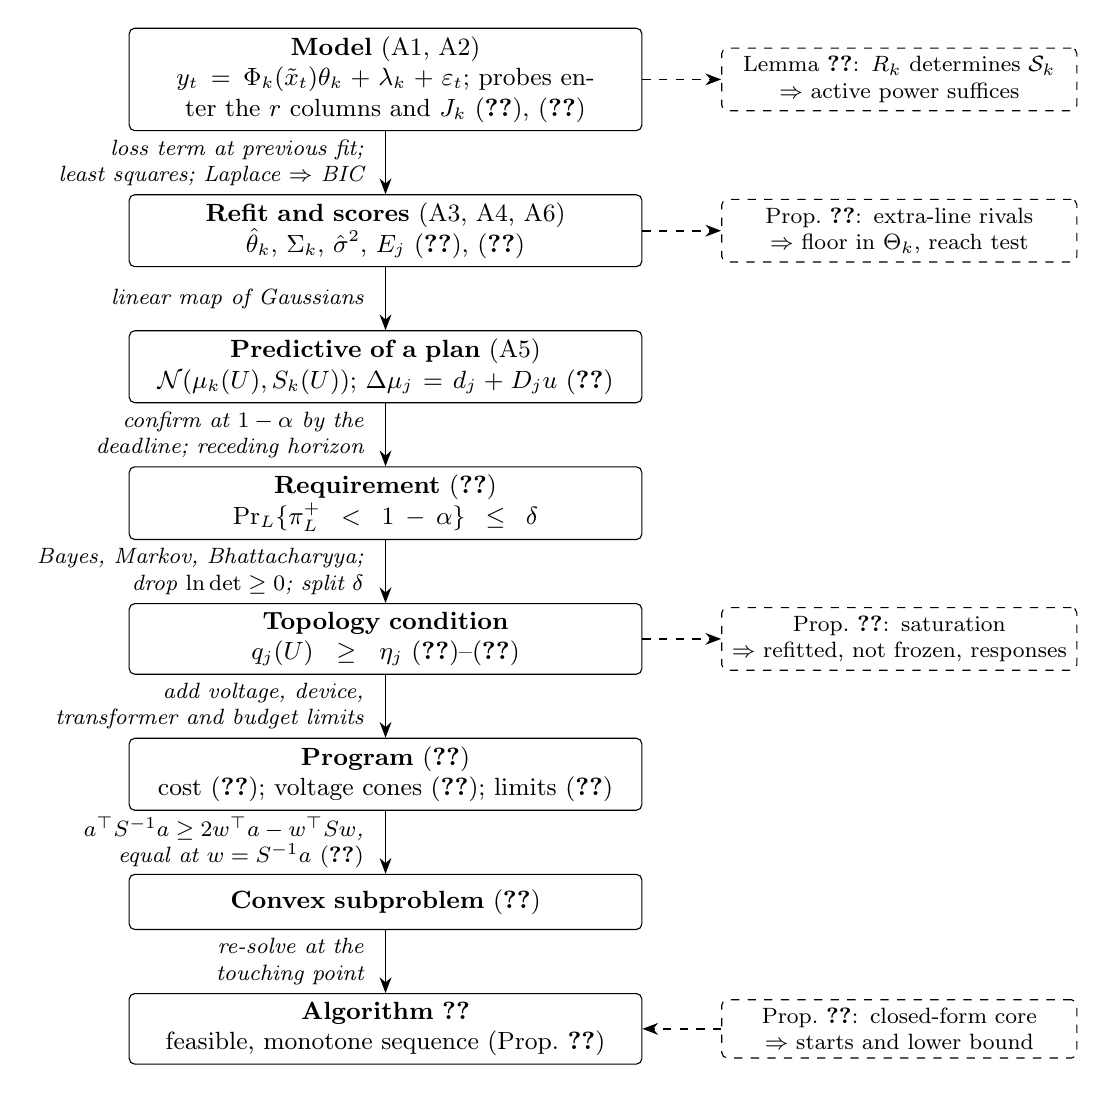
\begin{tikzpicture}[
  node distance=8mm and 10mm,
  main/.style={draw, rounded corners=2pt, align=center, text width=6.3cm, minimum height=7mm, inner sep=3pt, font=\small},
  side/.style={draw, dashed, rounded corners=2pt, align=center, text width=4.3cm, inner sep=3pt, font=\footnotesize},
  lab/.style={font=\footnotesize\itshape, align=right, anchor=east, xshift=-1.5mm},
  arr/.style={-{Stealth[length=2mm]}, semithick}
]
\node[main] (m1) {\textbf{Model} (A1, A2)\\ $y_t=\Phi_k(\tilde x_t)\theta_k+\lambda_k+\varepsilon_t$; probes enter the $r$ columns and $J_k$ \eqref{eq:model}, \eqref{eq:probecols}};
\node[main, below=of m1] (m2) {\textbf{Refit and scores} (A3, A4, A6)\\ $\hat\theta_k$, $\Sigma_k$, $\hat\sigma^2$, $E_j$ \eqref{eq:refit}, \eqref{eq:bic}};
\node[main, below=of m2] (m3) {\textbf{Predictive of a plan} (A5)\\ $\Nrm(\mu_k(U),S_k(U))$; $\Delta\mu_j=d_j+D_ju$ \eqref{eq:pred}};
\node[main, below=of m3] (m4) {\textbf{Requirement} \eqref{eq:req}\\ $\Pr_L\{\pi_L^+<1-\alpha\}\le\delta$};
\node[main, below=of m4] (m5) {\textbf{Topology condition}\\ $q_j(U)\ge\eta_j$ \eqref{eq:union}--\eqref{eq:gamma}};
\node[main, below=of m5] (m6) {\textbf{Program} \eqref{eq:P}\\ cost \eqref{eq:contract}; voltage cones \eqref{eq:vsoc}; limits \eqref{eq:env}};
\node[main, below=of m6] (m7) {\textbf{Convex subproblem} \eqref{eq:Pi}};
\node[main, below=of m7] (m8) {\textbf{Algorithm~\ref{alg:ccp}}\\ feasible, monotone sequence (Prop.~\ref{prop:seq})};
\draw[arr] (m1) -- node[lab] {loss term at previous fit;\\ least squares; Laplace $\Rightarrow$ BIC} (m2);
\draw[arr] (m2) -- node[lab] {linear map of Gaussians} (m3);
\draw[arr] (m3) -- node[lab] {confirm at $1-\alpha$ by the\\ deadline; receding horizon} (m4);
\draw[arr] (m4) -- node[lab] {Bayes, Markov, Bhattacharyya;\\ drop $\ln\det\ge0$; split $\delta$} (m5);
\draw[arr] (m5) -- node[lab] {add voltage, device,\\ transformer and budget limits} (m6);
\draw[arr] (m6) -- node[lab] {$a\tp S^{-1}a\ge2w\tp a-w\tp Sw$,\\ equal at $w=S^{-1}a$ \eqref{eq:qt}} (m7);
\draw[arr] (m7) -- node[lab] {re-solve at the\\ touching point} (m8);
\node[side, right=of m1] (s1) {Lemma~\ref{lem:R}: $R_k$ determines $\mathcal S_k$\\ $\Rightarrow$ active power suffices};
\node[side, right=of m2] (s2) {Prop.~\ref{prop:extra}: extra-line rivals\\ $\Rightarrow$ floor in $\Theta_k$, reach test};
\node[side, right=of m5] (s5) {Prop.~\ref{prop:saturation}: saturation\\ $\Rightarrow$ refitted, not frozen, responses};
\node[side, right=of m8] (s8) {Prop.~\ref{prop:core}: closed-form core\\ $\Rightarrow$ starts and lower bound};
\draw[arr, dashed] (m1) -- (s1);
\draw[arr, dashed] (m2) -- (s2);
\draw[arr, dashed] (m5) -- (s5);
\draw[arr, dashed] (s8) -- (m8);
\end{tikzpicture}
\caption{Derivation outline. Solid boxes form the chain from physics to the algorithm, and every formula they cite is used by the final subproblem \eqref{eq:Pi} (Table~\ref{tab:necessity}). Arrow labels name the operation. Dashed boxes are results that explain a design choice (Lemma~\ref{lem:R}, Propositions~\ref{prop:saturation} and~\ref{prop:extra}) or serve the algorithm without changing \eqref{eq:Pi} (Proposition~\ref{prop:core}).}\label{fig:skeleton}
\end{figure}

\begin{table}[!htbp]
\centering
\caption{Where each term of the final subproblem \eqref{eq:Pi} comes from}\label{tab:necessity}
\small
\begin{tabular}{@{}>{\raggedright\arraybackslash}p{3.8cm}>{\raggedright\arraybackslash}p{4.4cm}>{\raggedright\arraybackslash}p{3.1cm}>{\raggedright\arraybackslash}p{3.5cm}@{}}
\toprule
Term of \eqref{eq:Pi} & Meaning & Produced by & Status\\
\midrule
$\sum_\tau C_\tau(u_\tau)$ & Activation cost & \eqref{eq:contract} & Market rule\\
$\Delta\mu_j(U)=d_j+D_ju$ & Leader--rival difference of the predicted measurements under the plan, with operating-point sensitivities & \eqref{eq:model}, \eqref{eq:probecols}, \eqref{eq:refit}, \eqref{eq:pred} & Approximation (A1, A2, A5)\\
$\Phi_k(\hat X+U)$, $\Sigma_k$, $\hat\sigma^2$ & Regressors, parameter covariance and noise inside $\bar S_j$ & \eqref{eq:model}, \eqref{eq:refit}, \eqref{eq:bic} & Exact under A3, A4\\
$w_j^{(i)}$ & Touching point at the current plan & \eqref{eq:qt} & Exact\\
$\eta_j=8\gamma_j$ & Required level, from $E_j$, $\alpha$ and $\delta_j$ & \eqref{eq:req}--\eqref{eq:gamma}, \eqref{eq:bic} & Bound on the safe side; $E_j$ by BIC (A6)\\
$\mathcal A_h$, $\mathcal K_h$ & Active rivals; plausible candidates & \eqref{eq:bic}, \eqref{eq:equiv}, \eqref{eq:union} & Rule\\
Voltage cones & Chance constraint under every $k\in\mathcal K_h$ & \eqref{eq:vsoc} & First order; margin $\mu$; AC check\\
Device, energy, transformer, linearisation and budget limits & Deliverable activations & \eqref{eq:env}, \eqref{eq:P4}, \eqref{eq:P5} & Relaxation a cluster can deliver\\
\bottomrule
\end{tabular}
\end{table}

\emph{What is not needed for \eqref{eq:Pi}.} Three groups of formulas are kept but lie off the chain. (i) The regime rules \eqref{eq:equiv}--\eqref{eq:lm} decide when to plan and when to stop; they supply $\mathcal A_h$ and $\mathcal K_h$ but no term of \eqref{eq:Pi}. (ii) The restricted planner \eqref{eq:dict} and its excitation window \eqref{eq:kA}--\eqref{eq:kmax}, which the protocol uses by default, solve \eqref{eq:P} over a finite set of rays with the same topology condition; Algorithm~\ref{alg:ccp} uses their plan as one start. (iii) Lemma~\ref{lem:R}, Proposition~\ref{prop:saturation} and Proposition~\ref{prop:extra} explain why active power suffices, why the condition uses refitted rather than frozen responses, and why the refit keeps a resistance floor and the planner a reach test \eqref{eq:reach}. Standard steps (the branch-flow equations, Bayesian least squares, BIC as a Laplace approximation, the Bhattacharyya distance between Gaussians) are cited, not derived.

% ---------------------------------------------------------------------
\section{System Model}

\subsection{Network and measurement}
We use the branch-flow model in squared voltages \cite{baran1989}. Summing its branch equations along each root path cancels the intermediate voltages, and for a balanced radial feeder the result is exact (A1). For candidate $k$ and each 15-min sample,
\begin{equation}\label{eq:model}
\begin{gathered}
y_t=\sum_{C\in\mathcal S_k} z_C\big(r_C\,z_C\tp\tilde p_t+x_C\,z_C\tp\tilde q_t\big)+\lambda_k(\tilde x_t;\theta_k)+\varepsilon_t
=\Phi_k(\tilde x_t)\,\theta_k+\lambda_k(\tilde x_t;\theta_k)+\varepsilon_t,\\
R_k=\sum_{C\in\mathcal S_k}r_C\,z_Cz_C\tp,\qquad
\Phi_k(x)=\Big[\big(z_Cz_C\tp p\big)_{C\in\mathcal S_k}\ \Big|\ \big(z_Cz_C\tp q\big)_{C\in\mathcal S_k}\Big],\\
\lambda_k(x;\theta)=\sum_{C\in\mathcal S_k}z_C\Big(r_CL^P_C+x_CL^Q_C-\tfrac14\big(r_C^2+x_C^2\big)\ell_C\Big),\\
L^P_C=\tfrac12\!\!\sum_{C'\subseteq C}\!r_{C'}\ell_{C'},\quad
\ell_C=\frac{(z_C\tp p+L^P_C)^2+(z_C\tp q+L^Q_C)^2}{v_C^2},
\end{gathered}
\end{equation}
where $z_C\in\{0,1\}^n$ marks the terminals downstream of branch $C$, $r_C=2R_C^{\Omega}/Z_{\rm base}$ ($x_C$, $X_k$ and $L^Q_C$ likewise), $\theta_k$ has $p_k=2|\mathcal S_k|$ entries, and $\tilde x_t=(\tilde p_t,\tilde q_t)$ are the \emph{metered} injections, including probes and any locally controlled inverter reactive power (A2). $[R_k]_{ij}$ is the resistance of the path that $i$ and $j$ share. The loss term $\lambda_k$ is second order in the flows: $\ell_C$ is the squared current of branch C, and $L^P_C$, $L^Q_C$ are the losses that the branch carries for its downstream branches. The linearised model drops $\lambda_k$. Here it is kept, because it is a systematic, load-dependent error rather than noise, and because it has the support structure of the linear part, so it is exact for the true candidate. The flows are accumulated from the leaves upwards, and $v_C$ is taken from the candidate's linear prediction, which leaves an error of third order. A delivery shortfall $a\odot u$, $a\in[0.9,1]$, weakens the excitation but does not bias the fit, because the model uses metered injections. For an active-power probe $u$,
\begin{equation}\label{eq:probecols}
\begin{gathered}
\Phi_k\big((p+u,q)\big)=\Phi_k\big((p,q)\big)+\big[\,\Phi^r_k(u)\ \big|\ 0\,\big],\qquad
\Phi^r_k(u)=\big[\,z_{C}z_{C}\tp u\,\big]_{C\in\mathcal S_k},\\
\lambda_k\big((p+u,q)\big)=\lambda_k\big((p,q)\big)+J_k(p,q)\,u+O(\|u\|^2),\qquad J_k=\partial\lambda_k/\partial p,
\end{gathered}
\end{equation}
so probes change the $r$ columns and, through $J_k$, the loss term. The probe sensitivity of candidate $k$ is $R_k+J_k(\tilde x_t)$, which moves with the operating point. On branch $C$ the leading part of $J_k$ is $2|Z_C|^2P_C/v_C^2$, a fraction $(r_C^2+x_C^2)P_C/(2r_Cv_C^2)$ of the branch's own sensitivity $r_C$, with $Z_C$ the branch impedance and $P_C$ its flow. For the case feeders' backbone cable this fraction is about $0.87\,L_CP_C$ ($L_C$ in km, $P_C$ in pu), or 1--6\% on the head segment between mean and peak load. When planning, $\lambda_k$ is linearised at the forecast background $\hat x_t$. What the linearisation leaves out at terminal $j$ is
\begin{equation}\label{eq:rho}
\rho_j(u_t)\approx\sum_{C\ni j}\frac{|Z_C|^2}{\hat v^2}\big(2\bar\xi_{C,t}+|z_C\tp u_t|\big)\,|z_C\tp u_t|,
\end{equation}
where $\bar\xi_{C,t}$ is the $2\sigma$ forecast-error band of the flow $z_C\tp p_t$. The first term is the cross term of the probe with the forecast error, the second the probe's own square; \eqref{eq:P4} keeps $\rho_j$ below the noise level $\sigma_e$. Without $\lambda_k$ in the model, the cross term would involve the whole background flow $z_C\tp\hat p_t$ instead of its forecast error, and it would usually dominate.

\subsection{Controllable resources}
Each meter node is a cluster of household equivalents behind one service point. An aggregator dispatches enrolled household batteries and EV chargers device by device, so it can deliver node-specific active-power blocks within
\begin{equation}\label{eq:env}
-A_i^{-}\le u_i\le A_i^{+},\qquad
e_i(h+1)=e_i(h)+\Delta t\,\eta_i\,u_{i,b}(h),\qquad 0.2\,\bar e_i\le e_i(h)\le 0.8\,\bar e_i,
\end{equation}
where $u_{i,b}$ is the battery part of the block and $\eta_i$ its efficiency. Reactive power is not dispatched. Household inverters keep the default local volt-var response, which is zero between 220 and 240~V (about 0.953--1.039~pu on a 230.9~V base) \cite{asnzs4777}. Probes are kept inside this deadband, and any inverter reactive power that occurs is metered and enters \eqref{eq:model}.

\subsection{Market, contract and timing}
The operator buys P blocks and zero-sum P swaps. Activation is paid through the quadratic contract
\begin{equation}\label{eq:contract}
C_h(u)=\Delta t\sum_i c_i\left(\frac{(u_i^+)^2}{A_i^+}+\frac{(u_i^-)^2}{A_i^-}\right).
\end{equation}
Here $u_i^\pm\ge0$ are the upward and downward activations requested at node $i$, with $u_i=u_i^+-u_i^-$; both are paid. Blocks for hour $h+1$ are sealed at the start of hour $h$, with data up to the end of hour $h-1$.

% ---------------------------------------------------------------------
\section{Posterior and Scores}
Each candidate is refitted on all data by bounded least squares on its fixed supports, warm-started from its previous fit $\hat\theta_k^-$. Its loss term is evaluated at $\hat\theta_k^-$ and subtracted, a fixed-point step that keeps the refit a QP; with warm starts one step per hour suffices, and three are used at the first gate. With Gaussian noise (A3) and a flat prior, the parameter posterior is Gaussian on the free coordinates (A4):
\begin{equation}\label{eq:refit}
\hat\theta_k=\arg\min_{\theta\in\Theta_k}\ \mathrm{SSE}_k(\theta)=\sum_t\big\|y_t-\lambda_k(\tilde x_t;\hat\theta_k^-)-\Phi_k(\tilde x_t)\theta\big\|^2,\qquad
\theta_k\mid\mathcal D,k\sim\Nrm\big(\hat\theta_k,\Sigma_k\big),\quad
\Sigma_k=\hat\sigma^2\big(\Phi_k\tp\Phi_k\big)^{-1},
\end{equation}
with $\Phi_k$ the regressor stacked over all samples. The set $\Theta_k$ keeps the passive identifier's box bounds and adds the resistance floor $r_C\ge r_{\min}=2R_{\min}/Z_{\rm base}$ on every non-singleton support, with $R_{\min}$ the shortest internal segment resistance the operator's records allow (default $0.003~\Omega$). The floor is a bound, not a deletion: a branch at its floor stays in the candidate, so a candidate with an extra line remains the hypothesis that the line exists and is at least $R_{\min}$, and coordinates at a bound are left out of $\Sigma_k$. Reactance has no floor, because P-only probes inform only the resistance block. Proposition~\ref{prop:extra} shows why the floor matters. The dependence of $\lambda_k$ on $\theta$ would change $\Sigma_k$ by a relative amount of the order of the loss fraction above, and it is ignored. New data lower $\Sigma_k$ in the Loewner order. The topology weight is the marginal likelihood $p(\mathcal D\mid k)$, with the parameters integrated out rather than plugged in; a plug-in score drops the Occam factor and favours spurious splits. Its large-sample (Laplace) form is the Schwarz criterion \cite{schwarz1978} (A6):
\begin{equation}\label{eq:bic}
J_k=\frac{\mathrm{SSE}_k(\hat\theta_k)}{2\hat\sigma^2}+\frac{p_k}{2}\ln N,\qquad
\hat\sigma^2=\min_k\frac{\mathrm{SSE}_k}{N-p_k},\qquad
\pi_k\propto\pi_k^0e^{-J_k},\qquad E_j=J_j-J_L,
\end{equation}
with $N$ the number of scalar residuals and $L=\arg\min_kJ_k$. The within-topology part of the posterior covariance (R/X accuracy) is reported, not purchased: the topology decision integrates over it (Proposition~\ref{prop:saturation}), and reactance cannot be excited without reactive power.

% ---------------------------------------------------------------------
\section{Per-Gate Dispatch Program}\label{sec:program}

\subsection{Requirement}
The exact problem, which minimises the expected cost plus penalties for a wrong confirmation and for delay over a belief state on 40--60 topologies, is a partially observed control problem and is not solved. Its penalties are replaced by thresholds. A leader is confirmed only when $\pi_L\ge1-\alpha$, so under A7 a confirmation is wrong with posterior probability at most $\alpha$. At each gate the operator plans the hours $\mathcal H=\{h+1,\dots,h+T_r\}$ up to a rolling confirmation target, $T_r=\min\{H_c,\,T_{\max}-h\}$ with $H_c=2$~h by default and $T_{\max}$ the end of the probing day. It executes only the first block, and requires that the plan make the leader confirmable by the end of $\mathcal H$:
\begin{equation}\label{eq:req}
\Pr\nolimits_L\big\{\pi_L^+<1-\alpha\big\}\le\delta ,
\end{equation}
where $\pi_L^+$ is the posterior after the planned data $y_{\mathcal H}$ and $\Pr_L$ is taken under the leader's predictive distribution. If the leader is wrong, the data move the posterior and the next gate re-plans. The target $H_c$ sets the pace of probing: against a distant deadline, the background alone can meet \eqref{eq:req}, and nothing would be bought.

\subsection{Predictive distribution of a plan}
Let $U=(u_\tau)_{\tau\in\mathcal H}$ and $u=\vect U$, let $\hat X$ stack the forecast background samples, and let $\Phi_k(\hat X+U)$ stack the regressors of the planned samples, with probes in the P channels only. Under candidate $k$ (A5),
\begin{equation}\label{eq:pred}
\begin{gathered}
y_{\mathcal H}\mid\mathcal D,k\ \sim\ \Nrm\big(\mu_k(U),S_k(U)\big),\qquad
\mu_k(U)=\Phi_k(\hat X+U)\,\hat\theta_k+\lambda_k(\hat X)+J_k(\hat X)\,u,\qquad
S_k(U)=\hat\sigma^2I+\Phi_k(\hat X+U)\,\Sigma_k\,\Phi_k(\hat X+U)\tp,\\
\Delta\mu_j(U)=\mu_L(U)-\mu_j(U)=d_j+D_ju,
\end{gathered}
\end{equation}
where $\lambda_k$ and $J_k$ are evaluated at $\hat\theta_k$, $d_j=\Delta\mu_j(0)$ is the leader--rival difference under the forecast background alone, and $D_j$ applies the operating-point difference $\Delta R_{j,t}=R_L(\hat\theta_L)+J_L(\hat x_t)-R_j(\hat\theta_j)-J_j(\hat x_t)$ to the probe of planned sample $t$, by \eqref{eq:probecols}. $\mu_k$ is affine in $U$, and $S_k$ is a convex quadratic matrix function of $U$.

\subsection{Topology condition}
Let $p_k$ denote the predictive density \eqref{eq:pred} and $\Delta L_j=\ln p_L(y_{\mathcal H})-\ln p_j(y_{\mathcal H})$. By Bayes' rule, $\pi_L^+<1-\alpha$ if and only if $\sum_{j\ne L}e^{-E_j-\Delta L_j}>\alpha/(1-\alpha)$. Markov's inequality applied to the square root of this sum, and subadditivity of $\sqrt x$, give (Appendix~\ref{app:bound})
\begin{equation}\label{eq:union}
\begin{gathered}
\Pr\nolimits_L\{\pi_L^+<1-\alpha\}\le\sum_{j\ne L}c_j\,e^{-\mathcal B_j(U)},\\
c_j=\Big(\frac{1-\alpha}{\alpha}\Big)^{1/2}e^{-E_j/2},\qquad
\mathcal B_j(U)=-\ln\int\sqrt{p_L(y)\,p_j(y)}\,dy\ \ge\ 0 .
\end{gathered}
\end{equation}
$\mathcal B_j$ is the Bhattacharyya distance, the Chernoff divergence of order $\tfrac12$ \cite{chernoff1952}. For the Gaussian predictives \eqref{eq:pred} \cite{kailath1967},
\begin{equation}\label{eq:chernoff}
\begin{gathered}
\mathcal B_j(U)=\frac18\,q_j(U)+\frac12\ln\frac{\det\bar S_j}{(\det S_L\,\det S_j)^{1/2}}\ \ge\ \frac18\,q_j(U),\\
q_j(U)=\Delta\mu_j(U)\tp\bar S_j(U)^{-1}\Delta\mu_j(U),\qquad \bar S_j=\tfrac12\big(S_L+S_j\big).
\end{gathered}
\end{equation}
The log-determinant term is non-negative by concavity of $\ln\det$ and vanishes when $\Sigma=0$. It is the evidence carried by differences in predictive spread, which P-only probes barely create because only the resistance block of $\Sigma$ enters; dropping it is conservative. Split the failure probability as $\sum_{j\in\mathcal A_h}\delta_j=\delta-R_{\rm tail}$, where $R_{\rm tail}=\sum_{j\notin\mathcal A_h}c_j$ bounds the inactive rivals for every $U$ because $\mathcal B_j\ge0$. The active set $\mathcal A_h$ takes the non-equivalent rivals within probing reach \eqref{eq:reach} in increasing $E_j$ until $R_{\rm tail}\le\delta/2$, and the rest of $\delta=0.1$ is split equally, so $\delta_j\in[0.017,0.1]$ for one to three active rivals. Then the condition
\begin{equation}\label{eq:gamma}
q_j(U)\ \ge\ \eta_j:=8\gamma_j,\qquad
\gamma_j=\ln\frac{c_j}{\delta_j}=\frac12\Big(\ln\frac{1-\alpha}{\alpha}-E_j\Big)+\ln\frac{1}{\delta_j},
\end{equation}
for every $j\in\mathcal A_h$ guarantees \eqref{eq:req}; for $\alpha=0.05$ the bracket is $\ln19-E_j$. Any Chernoff order $\omega\in(0,1)$ gives a valid bound; order $\tfrac12$ is used, and in the frozen single-rival case the best order lowers the required information by less than 5\% for the settings of Section~\ref{sec:quality}. With known parameters, $q_j=\|\Delta\mu_j\|^2/\hat\sigma^2$ and \eqref{eq:gamma} is the quadratic constraint of frozen-parameter designs (Proposition~\ref{prop:saturation}).

\subsection{Voltage safety}
From $v_j=(v_0^2-y_j)^{1/2}$, the probe changes the voltage by $\Delta v_{j,t}\approx-\big(\phi_{kj}(u_t)\tp\theta_k+[J_k(\hat x_t)u_t]_j\big)/(2\hat v_j)$ to first order, where $\phi_{kj}(u)\tp$ is row $j$ of $[\Phi^r_k(u)\,|\,0]$. Under \eqref{eq:refit} this change is Gaussian with mean $g_{kj}(u_t)=-\big(\phi_{kj}(u_t)\tp\hat\theta_k+[J_k(\hat x_t)u_t]_j\big)/(2\hat v_j)$ and standard deviation $\beta_{kj}(u_t)=\|\Sigma_k^{1/2}\phi_{kj}(u_t)\|/(2\hat v_j)$; only the resistance block of $\Sigma_k$ enters. For single-phase blocks both are multiplied by 6, the phase-voltage allowance used until a three-phase model is available. The chance constraint with level $1-\epsilon_V$ is therefore the second-order cone pair
\begin{equation}\label{eq:vsoc}
\hat v^{+}_{j,t}+g_{kj}(u_t)+z\,\beta_{kj}(u_t)\le\bar v-\mu,\qquad
\hat v^{-}_{j,t}+g_{kj}(u_t)-z\,\beta_{kj}(u_t)\ge\underline v+\mu,
\end{equation}
for all $k\in\mathcal K_h$, with $\hat v^\pm$ the forecast $\pm2\sigma$ band, $z=F^{-1}(1-\epsilon_V)=2.33$ for $\epsilon_V=0.01$ ($F$ the standard normal distribution function), and the effective band $[\underline v+\mu,\bar v-\mu]=[0.96,1.035]$~pu, whose top edge keeps household volt-var inside its deadband. Because new data lower $\Sigma_k$, the cones can only widen as data accrue.

\subsection{The program}
\begin{subequations}\label{eq:P}
\begin{alignat}{2}
\min_{U}\quad & \sum_{\tau\in\mathcal H}C_\tau(u_\tau) && \label{eq:P1}\\
\text{s.t.}\quad & q_j(U)\ \ge\ \eta_j, && \quad j\in\mathcal A_h, \label{eq:P2}\\
& \text{the cones \eqref{eq:vsoc}}, && \quad k\in\mathcal K_h,\ \forall j,t, \label{eq:P3}\\
& u_\tau\in\mathcal U_\tau^{\dev}\ \text{by \eqref{eq:env}},\quad (P_{0,t}+\mathbf 1\tp u_t)^2+Q_{0,t}^2\le\bar S^2,\quad \rho_j(u_t)\le\sigma_e, && \quad \forall\tau,t,j, \label{eq:P4}\\
& C_\tau(u_\tau)\le B_h,\quad \sum_{\tau}C_\tau(u_\tau)\le B-B^{\rm spent}. && \label{eq:P5}
\end{alignat}
\end{subequations}
The objective is the contract cost \eqref{eq:contract}; information enters as a constraint, which by \eqref{eq:union}--\eqref{eq:gamma} implies \eqref{eq:req}. The solution is the cheapest safe purchase that makes the leader confirmable by the deadline with probability at least $1-\delta$. $\mathcal A_h$ and $\mathcal K_h$ come from the regime step (Section~\ref{sec:loop}). If \eqref{eq:P} is infeasible, a penalised slack on \eqref{eq:P2} turns it into ``most progress per unit cost''.

% ---------------------------------------------------------------------
\section{Solving the Program}\label{sec:nonconvex}

\subsection{Sources of nonconvexity}
Table~\ref{tab:nonconvex} lists six sources of nonconvexity. Modelling choices remove five; only the topology condition \eqref{eq:P2} needs an algorithm.

\begin{table}[!htbp]
\centering
\caption{Sources of nonconvexity and their treatment}\label{tab:nonconvex}
\small
\begin{tabular}{>{\raggedright\arraybackslash}p{2.5cm}>{\raggedright\arraybackslash}p{3.3cm}>{\raggedright\arraybackslash}p{6.0cm}>{\raggedright\arraybackslash}p{2.5cm}}
\toprule
Source & Why nonconvex & Treatment & Status\\
\midrule
Sequential decision & Belief-state control over 40--60 topologies & Thresholds $\alpha$, $\delta$, $T_{\max}$ and caps replace the penalties; receding horizon \eqref{eq:req} & Approximation\\
Topology choice & Discrete & Finite bank, enumerated; $\pi_k$ in closed form; no integer variables in \eqref{eq:P} & Exact\\
$H_k(\theta)\tilde x$ & Bilinear & $\hat\theta_k,\Sigma_k$ fixed at the gate and $\theta$ integrated out, so $\mu_k$ is affine and $S_k$ convex quadratic in $U$; the hourly refit is a convex QP on fixed supports, with the loss term fixed at the previous fit & Exact under the Gaussian model\\
AC power flow & Nonconvex equalities & Branch-flow model with the loss term fixed at the previous fit and linearised at the forecast in planning; margin $\mu$; remainder \eqref{eq:rho} limited in \eqref{eq:P4}; every executed block checked in AC & Approximation, checked\\
Device granularity & One battery cannot charge and discharge at once; EV charging has a 6~A minimum & Continuous node envelope with paid activations $u_i^\pm\ge0$; using both means two batteries in a cluster; EV requests rounded towards zero, re-checked, residual metered & Deliverable relaxation; no fit bias\\
Topology condition \eqref{eq:P2} & $q_j$ is convex when $\Sigma=0$, so \eqref{eq:P2} is reverse-convex; with $\Sigma\ne0$ it is neither convex nor concave & Convex restriction \eqref{eq:Pi} that touches \eqref{eq:P2}; sequence (Prop.~\ref{prop:seq}); starts and lower bound from the core problem (Prop.~\ref{prop:core}) & Local optimum; gap reported\\
\bottomrule
\end{tabular}
\end{table}

\subsection{Convex restriction}
For $S\succ0$ and any $w$, expanding the square gives \cite{boyd2004,shen2018}
\begin{equation}\label{eq:qt}
2w\tp a-w\tp Sw=a\tp S^{-1}a-\big(w-S^{-1}a\big)\tp S\,\big(w-S^{-1}a\big)\ \le\ a\tp S^{-1}a,
\end{equation}
with equality if and only if $w=S^{-1}a$. With $a=\Delta\mu_j(U)$ and $S=\bar S_j(U)$, define for a fixed $w$
\begin{equation}\label{eq:minor}
s_j(U;w)=2w\tp\Delta\mu_j(U)-\hat\sigma^2\|w\|^2-\tfrac12\big\|\Sigma_L^{1/2}\Phi_L(\hat X+U)\tp w\big\|^2-\tfrac12\big\|\Sigma_j^{1/2}\Phi_j(\hat X+U)\tp w\big\|^2,
\end{equation}
which is $2w\tp\Delta\mu_j-w\tp\bar S_jw$. Three facts follow: (i) $s_j(U;w)\le q_j(U)$ for all $U$ and $w$; (ii) at $w_j^\star(U_i)=\bar S_j(U_i)^{-1}\Delta\mu_j(U_i)$, $s_j(U_i;w_j^\star)=q_j(U_i)$; (iii) the gradients in $U$ agree at $U_i$ (Appendix~\ref{app:seq}). Because $\Phi_k$ is linear in its argument, $s_j$ is affine minus squared norms of affine functions of $U$, so it is concave and $s_j\ge\eta_j$ is a convex (rotated second-order cone) constraint. The vector $w_j^\star$ is the whitened leader--rival disagreement, and the two norm terms subtract the part of it that parameter re-tuning can explain. The final optimisation problem, solved at iterate $U_i$, is
\begin{equation}\label{eq:Pi}
\begin{aligned}
U_{i+1}=\arg\min_{U}\quad & \sum_{\tau\in\mathcal H}C_\tau(u_\tau)\\
\text{s.t.}\quad & s_j\big(U;w_j^{(i)}\big)\ \ge\ \eta_j,\quad w_j^{(i)}=\bar S_j(U_i)^{-1}\Delta\mu_j(U_i),\qquad j\in\mathcal A_h,\\
& \eqref{eq:P3}\text{--}\eqref{eq:P5}.
\end{aligned}
\end{equation}

\emph{Why not a tangent plane.} With $\Sigma=0$, $s_j$ is affine in $U$ and \eqref{eq:Pi} uses the tangent half-space of the frozen condition: the convex--concave procedure \cite{lipp2016}. With $\Sigma\ne0$, $q_j$ is not convex, so a plane tangent to $q_j$ lies above it somewhere, and a plan that satisfies the plane can violate \eqref{eq:P2}. The surrogate $s_j$ is tangent too, but curved: it linearises only the mean difference, keeps the parameter-uncertainty terms exactly, and by (i) stays below $q_j$ everywhere.

\begin{proposition}[Sequence of convex programs]\label{prop:seq}
Let $U_0$ be feasible for \eqref{eq:P} and let $U_{i+1}$ solve \eqref{eq:Pi}. Then (a) every $U_i$ is feasible for \eqref{eq:P}; (b) the cost is non-increasing in $i$; (c) under Slater's condition for the subproblems, every limit point is a KKT point of \eqref{eq:P}. Global optimality is not implied.
\end{proposition}

\subsection{Starts and a lower bound}\label{sec:core}
The feasible set of \eqref{eq:P2} has separate lobes: a rival can be separated at one node or another, in one hour or another, with either sign, and the sequence stays in the lobe of its start. A relaxation with a closed-form global solution picks the lobe and bounds the cost. Since $\bar S_j\succeq\hat\sigma^2I$, $q_j(U)\le\|\Delta\mu_j(U)\|^2/\hat\sigma^2$; and since $(u_i^+)^2+(u_i^-)^2\ge u_i^2$, the cost satisfies $\sum_\tau C_\tau(u_\tau)\ge u\tp Wu$ with $W=\Delta t\,\diag\big(c_i/\max(A_i^+,A_i^-)\big)$ in each hour. Keeping one rival and dropping \eqref{eq:P3}--\eqref{eq:P5} gives the \emph{core problem}
\begin{equation}\label{eq:coreprob}
C_j^{\rm core}=\min_u\ u\tp Wu\quad\text{s.t.}\quad\|d_j+D_ju\|^2\ \ge\ \hat\sigma^2\eta_j .
\end{equation}

\begin{proposition}[Core problem]\label{prop:core}
(a) $C_j^{\rm core}$ is at most the cost of any plan feasible for \eqref{eq:P}, so
\begin{equation}\label{eq:gapcore}
C^{\rm LB}=\max_{j\in\mathcal A_h}C_j^{\rm core}\ \le\ C^\star\ \le\ C^{\rm seq},
\end{equation}
where $C^\star$ is the optimal cost of \eqref{eq:P} and $C^{\rm seq}$ the cost returned by Algorithm~\ref{alg:ccp}. (b) If $\|d_j\|^2\ge\hat\sigma^2\eta_j$, then $C_j^{\rm core}=0$. Otherwise the global minimiser of \eqref{eq:coreprob} is
\begin{equation}\label{eq:core}
u_j(\lambda)=\lambda\big(W-\lambda D_j\tp D_j\big)^{-1}D_j\tp d_j,
\end{equation}
where $\lambda\in(0,1/\nu_1)$ is the unique root of $\|d_j+D_ju_j(\lambda)\|^2=\hat\sigma^2\eta_j$ (when it exists; Appendix~\ref{app:core} treats the exception) and $\nu_1$ is the largest eigenvalue of $W^{-1}D_j\tp D_j$. If $d_j=0$, the minimiser is $u_j=\pm(\hat\sigma^2\eta_j/\nu_1)^{1/2}e_1$, with $e_1$ the top generalised eigenvector of $(D_j\tp D_j,W)$ scaled so that $e_1\tp We_1=1$, and $C_j^{\rm core}=\hat\sigma^2\eta_j/\nu_1$.
\end{proposition}

Both $W$ and $D_j\tp D_j$ are block diagonal over the hours, with blocks $W_\tau$ and $\sum_{t\in\tau}\Delta R_{j,t}\tp\Delta R_{j,t}$, so \eqref{eq:core} needs only $n\times n$ solves: in hour $\tau$, $u_\tau=\lambda\big(W_\tau-\lambda\sum_{t\in\tau}\Delta R_{j,t}\tp\Delta R_{j,t}\big)^{-1}\sum_{t\in\tau}\Delta R_{j,t}\tp d_{j,t}$, where $d_{j,t}$ is the part of $d_j$ at sample $t$. The core plan therefore reinforces the leader--rival difference that the background already produces, mapped back through the sensitivity difference and weighted by price. It concentrates on the nodes at which the refitted sensitivities differ, which is where the dictionary's group blocks are placed, and for $d_j\ne0$ its sign is fixed.

\emph{Starts.} Algorithm~\ref{alg:ccp} starts from the core plan of each active rival, the dictionary plan \eqref{eq:dict}, and the previous plan shifted by one hour. Each start is first scaled along its ray to the smallest level that meets \eqref{eq:P2} for every active rival (a one-dimensional search), and is dropped if that level violates \eqref{eq:P3}--\eqref{eq:P5}; the dictionary plan already lies at that level. By Proposition~\ref{prop:seq}(b), the sequence never costs more than its scaled start. In particular, whenever the dictionary plan meets \eqref{eq:P2}, the returned plan costs no more than it, so $C^{\rm LB}\le C^{\rm seq}\le C^{\rm dict}$.

\emph{Gap.} The relative gap $(C^{\rm seq}-C^{\rm LB})/C^{\rm seq}$ is reported for every planned block. A small gap certifies that the plan is near-optimal for \eqref{eq:P}. A large gap is inconclusive, because it mixes local optimality with what the core problem ignores: saturation, the other rivals, unequal up and down headroom, and the limits \eqref{eq:P3}--\eqref{eq:P5}. The bound is exact when one rival is active, $A_i^+=A_i^-$, $\Sigma_k=0$ and the core plan meets \eqref{eq:P3}--\eqref{eq:P5}. A spatial branch-and-bound solver can bound the frozen program on small validation cases; \eqref{eq:P2} itself cannot be passed to such a solver, because it contains the inverse of a quadratic matrix function of $U$.

\subsection{Effort and quality}\label{sec:quality}
\emph{Effort.} The subproblem \eqref{eq:Pi} has $2nT_r$ non-negative variables (72 for $H_c=2$~h and $n\le18$; 432 for a 12-h target), two cones of size at most $p_k+2$ per active rival, and the voltage cones. Each $w_j^{(i)}$ needs one Cholesky factorisation of $\bar S_j(U_i)$, of size $mnT_r$ (144; 864), and each core plan one $n\times n$ generalised eigenproblem per hour. The restricted planner \eqref{eq:dict} needs a few dozen evaluations of $q_j$ per shape and rival, each one factorisation of the same size. Every iterate is feasible for \eqref{eq:P}, so the sequence can be stopped at any iteration, for example at the 60~s planning cap, and still returns a safe plan that meets \eqref{eq:req}. These sizes suggest seconds per gate with open-source conic solvers; this has not been measured.

\emph{What limits the cost of the plan.} Three things separate the returned cost from that of the cheapest plan meeting \eqref{eq:req}: local optimality, bounded by \eqref{eq:gapcore}; the dropped log-determinant term; and the bound \eqref{eq:union}--\eqref{eq:gamma} itself. Only the last can be computed in advance. In the frozen single-rival case, $\Delta L_j$ is Gaussian with mean $D$ and variance $2D$, where $D=q_j/2$. The exact form of \eqref{eq:req} is then $D-z_\delta\sqrt{2D}\ge\ln19-E_j$, with $z_\delta=F^{-1}(1-\delta_j)$, whereas \eqref{eq:gamma} asks for $D\ge2(\ln19-E_j)+4\ln(1/\delta_j)$. For $\ln19-E_j\in[1,3]$ and $\delta_j\in[0.017,0.1]$, the bound asks for 1.5--2.2 times the information, and hence the cost, of the exact constraint. This is the price of a guarantee that still holds when the parameters are uncertain, where $\Delta L_j$ is not Gaussian.

\begin{algorithm}[t]
\caption{Sequential convex solution of the dispatch program}\label{alg:ccp}
\begin{algorithmic}[1]
\Require active rivals $\mathcal A_h$; tolerance $\epsilon=10^{-4}$; $i_{\max}=20$
\State starts: the core plan \eqref{eq:core} of each $j\in\mathcal A_h$, the dictionary plan \eqref{eq:dict}, the previous plan shifted by one hour
\State scale each start along its ray to the smallest level meeting \eqref{eq:P2}; drop it if that level violates \eqref{eq:P3}--\eqref{eq:P5}
\For{each remaining start $U_0$}
  \State $i\gets0$
  \Repeat
    \State $w_j\gets\bar S_j(U_i)^{-1}\Delta\mu_j(U_i)$ for all $j\in\mathcal A_h$ \Comment{one Cholesky factorisation per rival}
    \State $U_{i+1}\gets$ solution of \eqref{eq:Pi};\quad $i\gets i+1$
  \Until{the relative cost decrease is below $\epsilon$ or $i=i_{\max}$}
\EndFor
\State keep the cheapest result; report its gap to $C^{\rm LB}$ \eqref{eq:gapcore}
\State \Return its first block $u_{h+1}$. If no start survives, solve \eqref{eq:Pi} with penalised slacks on its topology constraints (most progress per unit cost); on a solver failure, return the first block of the dictionary plan if it passes the checks, otherwise zero
\end{algorithmic}
\end{algorithm}

% ---------------------------------------------------------------------
\section{The PROBE Loop}\label{sec:loop}
Each hour runs five steps: \textbf{P}osterior, \textbf{R}egime, \textbf{O}ptimal design, \textbf{B}ound, \textbf{E}xecute (Algorithm~\ref{alg:probe}). The formulas of this section are not needed to state or solve \eqref{eq:Pi}: they decide when to plan and when to stop, and they define the restricted planner that the protocol uses by default.

\subsection{Regime: trigger, stopping, progress and guard}
Two candidates are operationally equivalent when their refitted voltage predictions over the forecast day differ by at most the meter resolution,
\begin{equation}\label{eq:equiv}
k\sim L\iff\max_{t,j}\big|\hat v^{(k)}_{j,t}-\hat v^{(L)}_{j,t}\big|\le\varepsilon_V .
\end{equation}
Probing is armed while a non-equivalent rival has $E_j<\ln19$. The leader is confirmed when
\begin{equation}\label{eq:stop}
\pi_L\ge1-\alpha\iff\sum_{j\ne L,\ j\nsim L}e^{-E_j}\le\frac{\alpha}{1-\alpha}
\end{equation}
holds for two consecutive hours; each pairwise term then satisfies Wald's bound $E_j\ge\ln\frac{1-\beta}{\alpha}=\ln19$ for $\alpha=\beta=0.05$ \cite{wald1945}. Let $G_h=\min_{j\in\mathcal A_h}E_j$. Buying stops for the day, and the input is reported as unresolved, when
\begin{equation}\label{eq:noprog}
G_h-G_{h-H_{\rm np}}<\Delta E_{\min}\quad\text{over the last } H_{\rm np} \text{ probed hours},\qquad H_{\rm np}=6,\ \Delta E_{\min}=1.
\end{equation}
For a nested extension of the leader with extra parameters $\psi$, the Rao score statistic \cite{rao1948}
\begin{equation}\label{eq:lm}
\mathrm{LM}=g_\psi\tp\big(\mathcal I_{\psi\psi}-\mathcal I_{\psi\theta}\mathcal I_{\theta\theta}^{-1}\mathcal I_{\theta\psi}\big)^{-1}g_\psi,\qquad g_\psi=\partial_\psi\ln\ell\,\big|_{\hat\theta_L,\psi=0},
\end{equation}
flags re-identification when $\mathrm{LM}>\chi^2_{2,0.99}=9.21$ for two consecutive hours.

\subsection{Optimal design: the restricted planner}
Every block of the restricted planner is written as $u=\kappa D_\sigma\bar s$ with $\|\bar s\|_\infty=1$, and a shape is held at one level over the planned hours, $U(\kappa;\bar s)=(\kappa D_\sigma\bar s,\dots,\kappa D_\sigma\bar s)$. The planner solves \eqref{eq:P} restricted to these rays. For each shape in a dictionary $\mathcal D_h$ it finds the smallest level that meets the topology condition \eqref{eq:P2}, and it keeps the cheapest shape whose level lies inside the excitation window \eqref{eq:kmax}:
\begin{equation}\label{eq:dict}
\kappa_{\rm need}(\bar s)=\min\big\{\kappa\ge0:\ q_j\big(U(\kappa;\bar s)\big)\ge\eta_j\ \ \forall j\in\mathcal A_h\big\},\qquad
\bar s_h=\arg\min_{\bar s\in\mathcal D_h:\ \kappa_{\rm need}(\bar s)\le\kappa_{\max}(\bar s)}\ \kappa_{\rm need}(\bar s)^2\,c(\bar s),
\end{equation}
where $c(\bar s)=\Delta t\sum_ic_i\sigma_i^2\bar s_i^2/A_i^{\pm}$ is the hourly cost at unit level by \eqref{eq:contract}, so the plan costs $T_r\kappa^2c(\bar s)$. The dictionary holds single-node $\pm$P blocks and group $\pm$P blocks on the nodes whose upstream path differs between the leader and an active rival. The search over $\kappa$ is one-dimensional: $q_j$ is evaluated on a grid of $[0,\kappa_{\max}(\bar s)]$, and the first crossing is refined by bisection. Along a ray $q_j$ need not be monotone, because a probe that opposes the background difference $d_j$ first lowers it. It can also stay below $\eta_j$ at every level when the two candidates can be made to agree along the shape (Proposition~\ref{prop:saturation}(b)); such a shape is not admissible. The block is zero if the background alone meets \eqref{eq:P2}. If no shape is admissible, the planner takes the shape with the largest $\min_jq_j/\eta_j$ at its ceiling $\kappa_{\max}(\bar s)$, the ray version of the slack fallback of \eqref{eq:P}.

\emph{Reach test.} Before $\mathcal A_h$ is formed, each non-equivalent rival is tested for whether the dictionary can still resolve it before the end of the day. Its reach
\begin{equation}\label{eq:reach}
\bar Q_j=\sum_{\tau=h+1}^{T_{\max}}\ \max_{\bar s\in\mathcal D_h}\ \max\big\{q^0_{j,\tau}(0),\ q^0_{j,\tau}\big(\bar\kappa_\tau(\bar s)D_\sigma\bar s\big)\big\},\qquad q^0_{j,\tau}=\|\Delta\mu_{j,\tau}\|^2/\hat\sigma^2,
\end{equation}
uses the frozen form of hour $\tau$ and the ceiling $\bar\kappa_\tau(\bar s)$ of that hour alone (headroom, voltage, transformer, unbalance and linearisation; energy and caps dropped). Because $\bar S_j\succeq\hat\sigma^2I$, $q_j\le q_j^0$; $q_j^0$ is additive over samples and convex along a ray, so its maximum on $[0,\bar\kappa_\tau]$ lies at an end. Hence $\bar Q_j$ bounds $q_j$ for every dictionary plan of the day, even one that changes shape every hour. A rival with $\bar Q_j<\eta_j$ at the most lenient share $\delta_j=\delta$ is beyond probing reach. It is left out of $\mathcal A_h$, and its $c_j$ is added to $R_{\rm tail}$; if these terms alone exceed $\delta/2$, the gate buys nothing. It stays in the stopping rule \eqref{eq:stop}, so its evidence comes only from the penalty and passive data. The typical case is the leader plus one extra branch held at its floor (Proposition~\ref{prop:extra}).

An admissible plan is feasible for \eqref{eq:P}, so it is a valid start of Algorithm~\ref{alg:ccp}. An optional mismatch check buys, in its first $H_{\rm chk}$ triggered hours, the broad zero-sum block
\begin{equation}\label{eq:check}
u^{\rm chk}_h=\varrho\,\diag(A)\,\tilde s_h,\qquad \mathbf 1\tp u^{\rm chk}_h=0,\qquad \varrho\le1,
\end{equation}
with random signs in $\tilde s_h$ rescaled so that buys and sells balance.

\subsection{Bound: the excitation window}\label{sec:window}
For a shape $\bar s$, every constraint of \eqref{eq:P3}--\eqref{eq:P5} is convex and holds at $\kappa=0$, so on the ray $\{U(\kappa;\bar s):\kappa\ge0\}$ it holds on an interval $[0,\kappa_\bullet(\bar s)]$, with each ceiling taken over all planned hours. The headroom ceiling is
\begin{equation}\label{eq:kA}
\kappa_A(\bar s)=\min_{i:\bar s_i\ne0}\frac{A_i^\pm}{\sigma_i|\bar s_i|},
\end{equation}
and $\kappa_E$, $\kappa_V$, $\kappa_S$, $\kappa_L$ and $\kappa_B$ are the ceilings from energy, the voltage cones \eqref{eq:vsoc}, the transformer, the linearisation limit and the caps \eqref{eq:P5}, for example $\kappa_L$, the positive root of $\max_{j,t}\rho_j(\kappa D_\sigma\bar s)=\sigma_e$ by \eqref{eq:rho}, and $\kappa_B=\min\big\{(B_h/c(\bar s))^{1/2},\,((B-B^{\rm spent})/(T_rc(\bar s)))^{1/2}\big\}$. For single-phase blocks, the 6-fold allowance in \eqref{eq:vsoc} gives $\kappa_U=\kappa_V/6$ in place of $\kappa_V$. The executed level is
\begin{equation}\label{eq:kmax}
\kappa_h=\min\{\kappa_{\rm need},\kappa_{\max}\},\qquad \kappa_{\max}=\min\{\kappa_A,\kappa_E,\kappa_V,\kappa_S,\kappa_L,\kappa_B\},
\end{equation}
where $\kappa_{\rm need}$ comes from \eqref{eq:dict}. An empty window, $\kappa_{\rm need}>\kappa_{\max}$, means that the enrolled resources cannot meet the requirement with this shape: change the shape, extend the deadline, or report that the rivals cannot be separated.

\begin{algorithm}[t]
\caption{PROBE, one feeder-day}\label{alg:probe}
\begin{algorithmic}[1]
\Require bank $\mathcal M$, passive fits, forecast, envelope \eqref{eq:env}, caps $B_h,B$, deadline $T_{\max}$
\State screen $\mathcal M$ with \eqref{eq:bic} and \eqref{eq:equiv}; if no rival is active, stay in Monitor
\For{each gate $h$ (data to the end of $h-1$; block for hour $h+1$)}
  \State \textbf{P:} refit all $k$ by \eqref{eq:refit}, warm-started; update $J_k,\pi_k,E_j,\Sigma_k$ by \eqref{eq:refit}--\eqref{eq:bic}
  \State \textbf{R:} guard \eqref{eq:lm}; stopping test \eqref{eq:stop}; no-progress test \eqref{eq:noprog}; reach test \eqref{eq:reach}; form $\mathcal K_h,\mathcal A_h$ ($u=0$ if $\mathcal A_h=\emptyset$)
  \State \textbf{O:} $U\gets$ \eqref{eq:check} in check hours; otherwise the dictionary plan \eqref{eq:dict}, refined by Algorithm~\ref{alg:ccp} when refinement is on
  \State \textbf{B:} check the first block against the window \eqref{eq:kmax}; otherwise fall back to the dictionary plan's first block, then to $0$
  \State \textbf{E:} submit $u_{h+1}$ to the aggregator; deliver; meter; cut on a voltage alarm; settle by \eqref{eq:contract}
\EndFor
\State \textbf{Output:} confirmed, undecided or unresolved topology; refitted $\hat H_L$ with $\Sigma_L$; cost ledger
\end{algorithmic}
\end{algorithm}

% ---------------------------------------------------------------------
\section{Properties}
The results of this section are not needed to state or solve \eqref{eq:Pi}; they explain three design choices.

\begin{lemma}[The structure is in $R$]\label{lem:R}
Let $\mathcal S$ be a laminar family that contains the singletons and the full set, and let $r_C>0$ for every $C\in\mathcal S$. Then $R=\sum_Cr_Cz_Cz_C\tp$ determines $\mathcal S$.
\end{lemma}
\begin{IEEEproof}[Proof sketch]
For a terminal $i$, the supports containing $i$ form a chain $C_1\supset C_2\supset\dots\supset\{i\}$ because the family is laminar. $R_{ij}$ is the sum of $r_C$ over the chain members that also contain $j$; since every $r_C>0$, it strictly increases with the depth of the deepest common support. The level sets $\{j:R_{ij}\ge c\}$ over the distinct values $c$ of row $i$ recover every member of the chain.
\end{IEEEproof}
Active-power probes, which reveal columns of $R$, can therefore identify the topology without reactive excitation; $X$ has the same supports and carries no additional structural information. By \eqref{eq:probecols}, the information that probes add lies in the $r$ block and grows as $\kappa^2$ for a probe of level $\kappa$; reactance is informed by passive data only.

\begin{proposition}[Frozen limit and saturation]\label{prop:saturation}
Assume the bounds are inactive.
\begin{enumerate}
\item[(a)] With $\Sigma_L=\Sigma_j=0$, $q_j(U)=\|\Delta\mu_j(U)\|^2/\hat\sigma^2$. Without the loss terms this is $\|(H_L-H_j)(\hat X+U)\|^2/\hat\sigma^2$, and \eqref{eq:P2} is the constraint $\|(H_L-H_j)(\hat X+U)\|^2/(8\hat\sigma^2)\ge\gamma_j$ of frozen-parameter procurement designs.
\item[(b)] Let $\hat X=0$ (a zero-mean code) and $U=\kappa V$, $v=\vect V$. Then $q_j(\kappa V)$ is non-decreasing in $\kappa$, $q_j(\kappa V)/\kappa^2$ is non-increasing and tends to the frozen value $\|D_jv\|^2/\hat\sigma^2$ as $\kappa\to0$, and for every $\kappa$, with $\|x\|_M^2=x\tp Mx$,
\[
q_j(\kappa V)\ \le\ 2\min\Big\{\|\theta_L'-\hat\theta_L\|^2_{\Sigma_L^{-1}}+\|\theta_j'-\hat\theta_j\|^2_{\Sigma_j^{-1}}\ :\ \Phi_L(V)\theta_L'=\Phi_j(V)\theta_j'\Big\},
\]
whereas the frozen form grows as $\kappa^2$. The bound is small when parameter changes that the passive data find plausible make the two candidates agree along $V$; for a rival that reproduces the leader, $\Phi_j(V)\theta'=\Phi_L(V)\hat\theta_L$, it is at most $2\|\theta'-\hat\theta_j\|^2_{\Sigma_j^{-1}}$.
\end{enumerate}
\end{proposition}
\begin{IEEEproof}[Proof sketch]
(a) Direct substitution. (b) With $a=D_jv$ and $A=\tfrac12\big(\Phi_L(V)\Sigma_L\Phi_L(V)\tp+\Phi_j(V)\Sigma_j\Phi_j(V)\tp\big)\succeq0$, $q_j(\kappa V)=a\tp(\hat\sigma^2\kappa^{-2}I+A)^{-1}a$, which increases with $\kappa$, and $q_j(\kappa V)/\kappa^2=a\tp(\hat\sigma^2I+\kappa^2A)^{-1}a$, which decreases. For any agreeing pair, $a=\Phi_L(V)b_L+\Phi_j(V)b_j$ with $b_L=\hat\theta_L-\theta_L'$ and $b_j=\theta_j'-\hat\theta_j$. By \eqref{eq:qt}, $q_j(\kappa V)=\max_w\{2w\tp a-w\tp(\hat\sigma^2\kappa^{-2}I+A)w\}$. Dropping the noise term and maximising separately over $z_L=\Phi_L(V)\tp w$ and $z_j=\Phi_j(V)\tp w$ bounds each part by $\max_z(2z\tp b-\tfrac12z\tp\Sigma z)=2b\tp\Sigma^{-1}b$.
\end{IEEEproof}
The topology condition therefore never certifies evidence that parameter re-tuning can explain, so uncalibrated reactance cannot create false topology evidence.

\begin{proposition}[Rivals with one extra line]\label{prop:extra}
Let rival $W$ be the leader $T$ plus one internal support $C_e$ with $n_e$ metered terminals and resistance column $\phi^r_e(x)=z_ez_e\tp p$, and let $G=\mathrm{SSE}_T-\mathrm{SSE}_W$, so that $E_W=\ln N-G/(2\sigma^2)$ by \eqref{eq:bic}. Let $T$ be true, \eqref{eq:model} exact, A3 hold with $\hat\sigma=\sigma$, and every bound other than those on $C_e$ be inactive.
\begin{enumerate}
\item[(a)] Without a floor ($r_e,x_e\ge0$), $W$ reproduces $T$ for every data set and every probe, so $G\ge0$, and
\begin{equation}\label{eq:extra}
\Pr\{E_W<\ln19\}\ \le\ \Pr\{\chi^2_2>2\ln(N/19)\}=\frac{19}{N}.
\end{equation}
\item[(b)] If the data contain an omitted error $b$, let $g$ be its part that $W$'s extra columns explain beyond $T$'s, with $\|g\|^2=N\beta^2\sigma^2$ and a sign the bounds allow. Then $\E\,G\ge\|g\|^2$, and $W$ leads $T$ by $\ln19$ in expectation once $\beta>\beta^\star=\sqrt{2(\ln N+\ln19)/N}$.
\item[(c)] With the floor $r_e\ge r_{\min}$ active, and up to the noise fitted by the free $x_e$, $\Delta\mu_W(U)=r_{\min}\,a_e(U)$. Here $a_e$, the part of $\phi^r_e$ that $W$'s free columns do not absorb on the fitted data, does not depend on $r_{\min}$, so $q_W(U)\le r_{\min}^2\|a_e(U)\|^2/\hat\sigma^2$.
\end{enumerate}
\end{proposition}
\begin{IEEEproof}[Proof sketch]
(a) Setting $r_e=x_e=0$ gives $T$. $G$ is the squared norm of the projection of the noise, orthogonalised against $T$'s columns, onto a closed convex cone of dimension at most two, so $G/\sigma^2$ is stochastically below $\chi^2_2$, whose survival function is $e^{-x/2}$. (b) Without bounds, $G=\|\Pi(b+\varepsilon)\|^2$ with $\Pi$ that projector, and its mean is $\|g\|^2+2\sigma^2$; a sign the bounds allow keeps the first term. Requiring $\E\,G/(2\sigma^2)\ge\ln N+\ln19$ gives $\beta^\star$. (c) Both candidates are fitted to the same data. With the other bounds inactive, $W$'s free coefficients equal those of its fit without $r_e$, minus $r_{\min}$ times the regression of $\phi^r_e$ on the free columns, so the predicted difference is linear in $r_{\min}$; $q_W\le\|\Delta\mu_W\|^2/\hat\sigma^2$ because $\bar S_W\succeq\hat\sigma^2I$.
\end{IEEEproof}
Against an extra-line rival the evidence therefore comes from the penalty, not from probing. By \eqref{eq:extra}, BIC leaves such a rival within $\ln19$ with probability at most $19/N$ (about 1\% at $N=2000$) without any probe; validation MSE gives no such protection. The protection holds only while the residual has no systematic part along the extra branch. Since $\beta^\star$ is 0.10 at $N=2000$ and 0.049 at $N=10\,000$, the loss term is kept and $b/J$ is reported by rival type.

By (c), the floor sets what probing can add. For a block inside the subtree of $C_e$, the probe part of $a_e$ is of the order of $\sqrt{n_e}\,|z_e\tp u_t|$ per sample. Take $R_{\min}=0.003~\Omega$ ($r_{\min}=0.0075$), $\hat\sigma=\sigma_e$ and 5--20~kW below the branch. A block then adds at most $n_e(0.07$--$1.15)$ to $q_W$ per hour, against $\eta_j=22$--45 for the settings of Section~\ref{sec:quality}. Meeting $\eta_j$ within $H_c=2$~h with 10~kW would need $R_{\min}\approx0.019$--$0.026~\Omega$. At $R_{\min}=0.003~\Omega$ such a rival moves the predicted voltage of a 10~kW subtree by about 0.04~V, below a 0.05\% meter class, so \eqref{eq:equiv} usually classes it as equivalent; otherwise the reach test \eqref{eq:reach} stops the planner from buying against it.

Result (a) uses A3. The shared root meter correlates the terminals' noise ($\rho\approx\tfrac12$ for equal meters), and its effect on \eqref{eq:extra} is not yet quantified.

\begin{remark}[Impedance scaling]
Multiply all branch impedances by $s$ and assume voltage-meter noise dominates $\sigma_e$. Then $d_j$ and $D_j$ scale with $s$, so the level needed for a given $q_j$ falls as $1/s$; $\kappa_A$ and $\kappa_S$ do not change; and $\kappa_V$ falls roughly as $1/s$ for upward pushes and faster for downward pushes, because the background drop also grows with $s$.
\end{remark}

% ---------------------------------------------------------------------
\section{Case-Study Parameters and Pre-Check (Summary)}
Two synthetic balanced LV feeders (11 and 18 terminals, 0.4~kV, 200~kVA base, impedance scale 1, feeders of at most 186~m) are used; full data and sources are in the accompanying manuscript. Each meter node is a cluster of $N_i=\bar p_i/0.8$~kW household equivalents (62 and 114 in total).

\begin{table}[h]
\centering
\caption{Resource scenarios and the headroom ceiling $\kappa_A$ (active power only)}
\begin{tabular}{@{}llrr@{}}
\toprule
Scenario & Resources & Day & Night\\
\midrule
R0 & Repository library & $<1$ & $<1$\\
R1 (main) & 25\% batteries (5~kW/13.5~kWh), 20\% EVs (7~kW), 25\% enrolled & 1.2--1.5 & 2.5--3.3\\
R1, low adoption & 10\% batteries, 5\% EVs, 25\% enrolled & 0.5--0.6 & 0.8--1.1\\
R2 & R1 plus one operator-owned battery at a mid-feeder node & \multicolumn{2}{r}{R1, plus one strong node}\\
\bottomrule
\end{tabular}
\end{table}

Household inverters keep local volt-var \cite{asnzs4777,cec2021}; transformers are rated 125 and 200~kVA; the probing band is $[0.96,1.035]$~pu. In a linear-model pre-check with uniform levels $\kappa=1.5$ and 3 and 20 seeds, targeted P probes confirmed the true topology in every run, in 2.9--4.8~h against 4.4--7.8~h for passive data, for 2--4~CNY per day, with reactance error left at 0.57--0.77. Scoring the same probes with the frozen passive fit confirmed a wrong topology in 15\% of runs on one feeder. With the truth missing from the bank, 35--40\% of passive and targeted runs confirmed a wrong topology; a broad zero-sum check lowered this to 5--20\% at 10--50 times the cost. The pre-check chose its shapes by the expected refit-aware evidence gain \cite{atkinson1975}, with the leader's prediction taken as exact, and aimed at an expected evidence of $\ln19-E_j$ within two hours. It therefore does not test the planner \eqref{eq:dict}, which asks for that evidence with probability at least $1-\delta_j$: in the frozen single-rival case, $2+4\ln(1/\delta_j)/(\ln19-E_j)$ times as much information, or 5--18 times for the settings of Section~\ref{sec:quality}. Its level is therefore 2.2--4.3 times higher, and under R1 the window \eqref{eq:kmax} may often be empty, in which case the planner runs its best shape at the ceiling. The pre-check was also linear, so it did not test the loss term. The study evaluates every block in AC and measures the remaining bias of the leader's prediction, $e$, against each planned leader--rival difference $d_j$ by $b/J=2\langle e,d_j\rangle/\|d_j\|^2$: at $b/J=-1$ the bias cancels the evidence.

Wrong confirmations and $b/J$ are reported by type relative to the truth: an extra line, a missing line, or a wrong placement. Extra-line rivals are shown separately, because a systematic error can make them win (Proposition~\ref{prop:extra}(b)). The development stage adds two variants. An unbalanced AC evaluation places households on single phases while the fit stays balanced; this needs a three-phase evaluator. A short-line set shortens one internal segment of the true network to $1.5R_{\min}$ and regenerates the bank, which measures the other error a floor can cause, a real short line that is missed.

% ---------------------------------------------------------------------
\appendices
\section{Proof of the Bound and the Level}\label{app:bound}
This appendix proves \eqref{eq:union} and \eqref{eq:gamma}. By Bayes' rule, $\pi_k^+\propto\pi_k\,p_k(y_{\mathcal H})$. Dividing by the leader's term,
\begin{equation}\label{eq:A1}
\pi_L^+=\Big(1+\sum_{j\ne L}e^{-E_j-\Delta L_j}\Big)^{-1},
\end{equation}
so $\pi_L^+<1-\alpha$ if and only if $R=\sum_{j\ne L}e^{-E_j-\Delta L_j}>a$, with $a=\alpha/(1-\alpha)$. Markov's inequality applied to $\sqrt R$, and $\sqrt{\textstyle\sum_jx_j}\le\sum_j\sqrt{x_j}$, give
\begin{equation}\label{eq:A2}
\Pr\nolimits_L\{R>a\}\le a^{-1/2}\,\E_L\big[\sqrt R\big]\le a^{-1/2}\sum_{j\ne L}e^{-E_j/2}\,\E_L\big[e^{-\Delta L_j/2}\big]=\sum_{j\ne L}c_j\,e^{-\mathcal B_j(U)},
\end{equation}
because $e^{-\Delta L_j/2}=(p_j/p_L)^{1/2}$ and hence $\E_L[e^{-\Delta L_j/2}]=\int\sqrt{p_Lp_j}\,dy=e^{-\mathcal B_j}$. By the Cauchy--Schwarz inequality this integral is at most 1, so $\mathcal B_j\ge0$. For Gaussian densities it has the closed form \eqref{eq:chernoff} \cite{kailath1967}, and the log-determinant term is non-negative because $\ln\det$ is concave: $\ln\det(\tfrac12S_L+\tfrac12S_j)\ge\tfrac12\ln\det S_L+\tfrac12\ln\det S_j$. For the level, let each active rival contribute at most $\delta_j$: $c_je^{-\mathcal B_j}\le\delta_j$ if and only if $\mathcal B_j\ge\gamma_j$, which \eqref{eq:gamma} implies through $\mathcal B_j\ge q_j/8$. Each inactive rival contributes at most $c_j$ for every $U$, so the bound is at most $\sum_{j\in\mathcal A_h}\delta_j+R_{\rm tail}=\delta$. This needs $R_{\rm tail}<\delta$; otherwise more rivals are activated.

\section{Proof of the Sequence Properties}\label{app:seq}
This appendix proves fact (iii) of Section~\ref{sec:nonconvex} and Proposition~\ref{prop:seq}.

\emph{Tangency.} Fix $w_i=w_j^\star(U_i)$. By \eqref{eq:qt}, $\psi(U)=q_j(U)-s_j(U;w_i)=\big(w_i-w_j^\star(U)\big)\tp\bar S_j(U)\big(w_i-w_j^\star(U)\big)\ge0$, and $\psi(U_i)=0$. A differentiable non-negative function that vanishes at $U_i$ has a minimum there, so $\nabla\psi(U_i)=0$: $s_j(\cdot\,;w_i)$ and $q_j$ have equal values and gradients at $U_i$.

(a) By fact (i), $s_j\ge\eta_j$ implies $q_j\ge\eta_j$, so every solution of \eqref{eq:Pi} is feasible for \eqref{eq:P}. (b) If $U_i$ is feasible for \eqref{eq:P}, then $s_j(U_i;w_j^{(i)})=q_j(U_i)\ge\eta_j$, so $U_i$ is feasible for \eqref{eq:Pi} and $U_{i+1}$ costs no more. (c) The cost is bounded below by zero, so it converges. The cost \eqref{eq:contract} is strictly convex in $(u^+,u^-)$, so each subproblem has a unique solution. Under Slater's condition, every limit point $\bar U$ is a fixed point: it solves \eqref{eq:Pi} at $w_j^\star(\bar U)$, and by tangency its KKT conditions are those of \eqref{eq:P} \cite{marks1978,lipp2016}.

\section{Proof of the Core Solution}\label{app:core}
This appendix proves Proposition~\ref{prop:core}.

(a) Each $S_k\succeq\hat\sigma^2I$, so $\bar S_j\succeq\hat\sigma^2I$ and $q_j(U)\le\|\Delta\mu_j(U)\|^2/\hat\sigma^2$; every plan feasible for \eqref{eq:P} therefore meets the constraint of \eqref{eq:coreprob}. Its cost is at least $u\tp Wu$, because
$(u_i^+)^2/A_i^++(u_i^-)^2/A_i^-\ge\big((u_i^+)^2+(u_i^-)^2\big)/\max(A_i^+,A_i^-)\ge u_i^2/\max(A_i^+,A_i^-)$.
Hence the cost of every such plan is at least $C_j^{\rm core}$ for each $j$, which gives \eqref{eq:gapcore}.

(b) Let $v=W^{1/2}u$ and $M=D_jW^{-1/2}$, with singular value decomposition $M=\sum_l\sigma_la_lb_l\tp$, $\nu_l=\sigma_l^2$ and $\xi_l=a_l\tp d_j$. Problem \eqref{eq:coreprob} becomes $\min\|v\|^2$ subject to $\|d_j+Mv\|^2\ge\hat\sigma^2\eta_j$: one quadratic objective and one quadratic constraint. If $M\ne0$, Slater's condition holds, the S-lemma gives zero duality gap, and $v$ is globally optimal if and only if, for some $\lambda\ge0$,
\begin{equation}\label{eq:A3}
(I-\lambda M\tp M)\,v=\lambda M\tp d_j,\qquad I-\lambda M\tp M\succeq0,
\end{equation}
with the constraint tight when $\lambda>0$ \cite[App.~B]{boyd2004}, \cite{more1983}. Hence $\lambda\le1/\nu_1$ and, for $\lambda<1/\nu_1$, $v(\lambda)=\sum_l\lambda\sigma_l\xi_l\,b_l/(1-\lambda\nu_l)$, so that
\begin{equation}\label{eq:A4}
\|d_j+Mv(\lambda)\|^2=\|d_j\|^2-\sum_l\xi_l^2+\sum_l\frac{\xi_l^2}{(1-\lambda\nu_l)^2}.
\end{equation}
This increases with $\lambda$ from $\|d_j\|^2$, strictly unless every $\xi_l$ vanishes, so the root is unique; it exists below $1/\nu_1$ when $\xi_1\ne0$. Transforming back, $u=W^{-1/2}v(\lambda)=\lambda(W-\lambda D_j\tp D_j)^{-1}D_j\tp d_j$, which is \eqref{eq:core}. If no root exists below $1/\nu_1$ (the hard case of trust-region problems \cite{more1983}), then $\lambda=1/\nu_1$ and a multiple of $b_1$ is added to $v$. With $d_j=0$, the constraint is $v\tp M\tp Mv\ge\hat\sigma^2\eta_j$, which is met at least cost by $v=\pm(\hat\sigma^2\eta_j/\nu_1)^{1/2}b_1$; this gives the last statement with $e_1=W^{-1/2}b_1$.

% ---------------------------------------------------------------------
\begin{thebibliography}{99}

\bibitem{cavraro2019}
G.~Cavraro and V.~Kekatos, ``Inverter probing for power distribution network topology processing,'' \emph{IEEE Trans. Control Netw. Syst.}, 2019, arXiv:1802.06027.

\bibitem{cavraro2018}
G.~Cavraro and V.~Kekatos, ``Graph algorithms for topology identification using power grid probing,'' \emph{IEEE Control Syst. Lett.}, 2018, arXiv:1803.04506.

\bibitem{taheri2020}
S.~Taheri, V.~Kekatos, and G.~Cavraro, ``An MILP approach for distribution grid topology identification using inverter probing,'' arXiv:2004.02370.

\bibitem{bhela2019}
S.~Bhela, V.~Kekatos, and S.~Veeramachaneni, ``Smart inverter grid probing for learning loads: Part~II---Probing injection design,'' \emph{IEEE Trans. Power Syst.}, vol.~34, pp.~3537--3546, 2019.

\bibitem{ieee1547}
\emph{IEEE Standard for Interconnection and Interoperability of Distributed Energy Resources with Associated Electric Power Systems Interfaces}, IEEE Std 1547-2018.

\bibitem{asnzs4777}
\emph{Grid connection of energy systems via inverters, Part~2: Inverter requirements}, AS/NZS 4777.2:2020.

\bibitem{cec2021}
Clean Energy Council, ``New inverter standard to improve grid stability,'' news release. [Online]. Available: \url{https://www.cleanenergycouncil.org.au/news/new-inverter-standard-to-improve-grid-stability}

\bibitem{ausnet2019}
AusNet Services, University of Technology Sydney \emph{et al.}, \emph{Networks Renewed: Public Dissemination Report}, Oct. 2019.

\bibitem{ausgrid2023}
Ausgrid, ``Community battery trial, Beacon Hill,'' conference presentation, 2023. [Online]. Available: \url{https://bsgip.com/wp-content/uploads/2023/12/Alan_Luc.pdf}

\bibitem{iou2018}
California investor-owned utilities, \emph{EPIC Project 2.03A: Joint IOU Smart Inverter White Paper, Appendix}.

\bibitem{jin2020}
X.~Jin, Q.~Wu, and H.~Jia, ``Local flexibility markets: Literature review on concepts, models and clearing methods,'' \emph{Applied Energy}, vol.~261, Art.~114387, 2020.

\bibitem{boxhill1967}
G.~E.~P. Box and W.~J. Hill, ``Discrimination among mechanistic models,'' \emph{Technometrics}, vol.~9, no.~1, pp.~57--71, 1967.

\bibitem{atkinson1975}
A.~C. Atkinson and V.~V. Fedorov, ``The design of experiments for discriminating between two rival models,'' \emph{Biometrika}, vol.~62, no.~1, pp.~57--70, 1975.

\bibitem{wald1945}
A.~Wald, ``Sequential tests of statistical hypotheses,'' \emph{Ann. Math. Statist.}, vol.~16, no.~2, pp.~117--186, 1945.

\bibitem{schwarz1978}
G.~Schwarz, ``Estimating the dimension of a model,'' \emph{Ann. Statist.}, vol.~6, no.~2, pp.~461--464, 1978.

\bibitem{sui2015}
Y.~Sui, A.~Gotovos, J.~Burdick, and A.~Krause, ``Safe exploration for optimization with Gaussian processes,'' in \emph{Proc. ICML}, 2015.

\bibitem{baran1989}
M.~E. Baran and F.~F. Wu, ``Network reconfiguration in distribution systems for loss reduction and load balancing,'' \emph{IEEE Trans. Power Del.}, vol.~4, no.~2, pp.~1401--1407, 1989.

\bibitem{chernoff1952}
H.~Chernoff, ``A measure of asymptotic efficiency for tests of a hypothesis based on the sum of observations,'' \emph{Ann. Math. Statist.}, vol.~23, no.~4, pp.~493--507, 1952.

\bibitem{kailath1967}
T.~Kailath, ``The divergence and Bhattacharyya distance measures in signal selection,'' \emph{IEEE Trans. Commun. Technol.}, vol.~15, no.~1, pp.~52--60, 1967.

\bibitem{boyd2004}
S.~Boyd and L.~Vandenberghe, \emph{Convex Optimization}. Cambridge, U.K.: Cambridge Univ. Press, 2004.

\bibitem{lipp2016}
T.~Lipp and S.~Boyd, ``Variations and extension of the convex--concave procedure,'' \emph{Optim. Eng.}, vol.~17, no.~2, pp.~263--287, 2016.

\bibitem{shen2018}
K.~Shen and W.~Yu, ``Fractional programming for communication systems---Part~I: Power control and beamforming,'' \emph{IEEE Trans. Signal Process.}, vol.~66, no.~10, pp.~2616--2630, 2018.

\bibitem{marks1978}
B.~R. Marks and G.~P. Wright, ``A general inner approximation algorithm for nonconvex mathematical programs,'' \emph{Oper. Res.}, vol.~26, no.~4, pp.~681--683, 1978.

\bibitem{more1983}
J.~J. Mor\'e and D.~C. Sorensen, ``Computing a trust region step,'' \emph{SIAM J. Sci. Stat. Comput.}, vol.~4, no.~3, pp.~553--572, 1983.

\bibitem{rao1948}
C.~R. Rao, ``Large sample tests of statistical hypotheses concerning several parameters with applications to problems of estimation,'' \emph{Proc. Cambridge Philos. Soc.}, vol.~44, pp.~50--57, 1948.

\end{thebibliography}

\end{document}
